Come backend di scansione si è adottato il framework di \textbf{Greenbone OpenVAS}.

In questo capitolo si vuole spiegare nel dettaglio la struttura e il funzionamento del sistema usato come base del progetto.

\section{Storia del progetto}
\textbf{OpenVAS} (\emph{Open Vulnerability Assessment Scanner}) è una piattaforma \emph{open source} per la rilevazione, l'analisi e la gestione di vulnerabilità e falle di sicurezza.

OpenVAS nasce nel 2005 come \emph{fork} dello scanner \textbf{Nessus}, quando quest'ultimo modificò la propria licenza, diventando un software proprietario distribuito sotto licenza commerciale. La comunità \emph{open source} ha quindi manutenuto il \emph{fork} risultante, inizialmente denominato \emph{GNessUs} e successivamente rinominato \emph{OpenVAS}. In seguito, il progetto è entrato a far parte delle iniziative supportate economicamente dalla \emph{Software in the Public Interest}.

\begin{figure}[h]
    \centering
    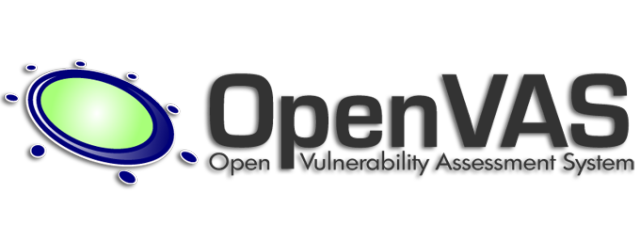
\includegraphics{img/openvas_logo.png}
    \caption{Logo originale del progetto OpenVAS}
\end{figure}

Tra i principali contributori iniziali del \emph{fork} figuravano gli sviluppatori di Intevation e DN-Systems, aziende che in seguito si sarebbero trasformate in Greenbone AG, finanziata anche dalla BSI tedesca (l'Ufficio Federale per la Sicurezza Informatica). Nel 2008, la neo-costituita Greenbone si pose l'obiettivo di sostenere lo sviluppo \emph{open source} di OpenVAS, creando al contempo versioni ottimizzate per clienti \emph{enterprise} e fornendo supporto commerciale.

Con il tempo, altre aziende hanno contribuito al progetto, garantendo un \emph{feed} stabile e aggiornato di test di vulnerabilità, una componente chiave del sistema. Nel 2010, OpenVAS ha rotto la compatibilità con Nessus, consolidando la propria identità indipendente. Negli anni successivi, ha ricevuto ulteriore supporto dalla BSI e dalla DFN (la rete di ricerca tedesca), che hanno contribuito pubblicando avvisi di sicurezza regolari sotto licenza GPL.

Nel 2017, i contributi di Greenbone sono diventati evidenti con un cambio di nome ufficiale: il progetto non è più noto come \emph{OpenVAS framework}, ma come \textbf{Greenbone Vulnerability Management (GVM)}. OpenVAS identifica ora esclusivamente lo scanner, che è uno dei molti componenti del framework.

\begin{figure}
    \centering
    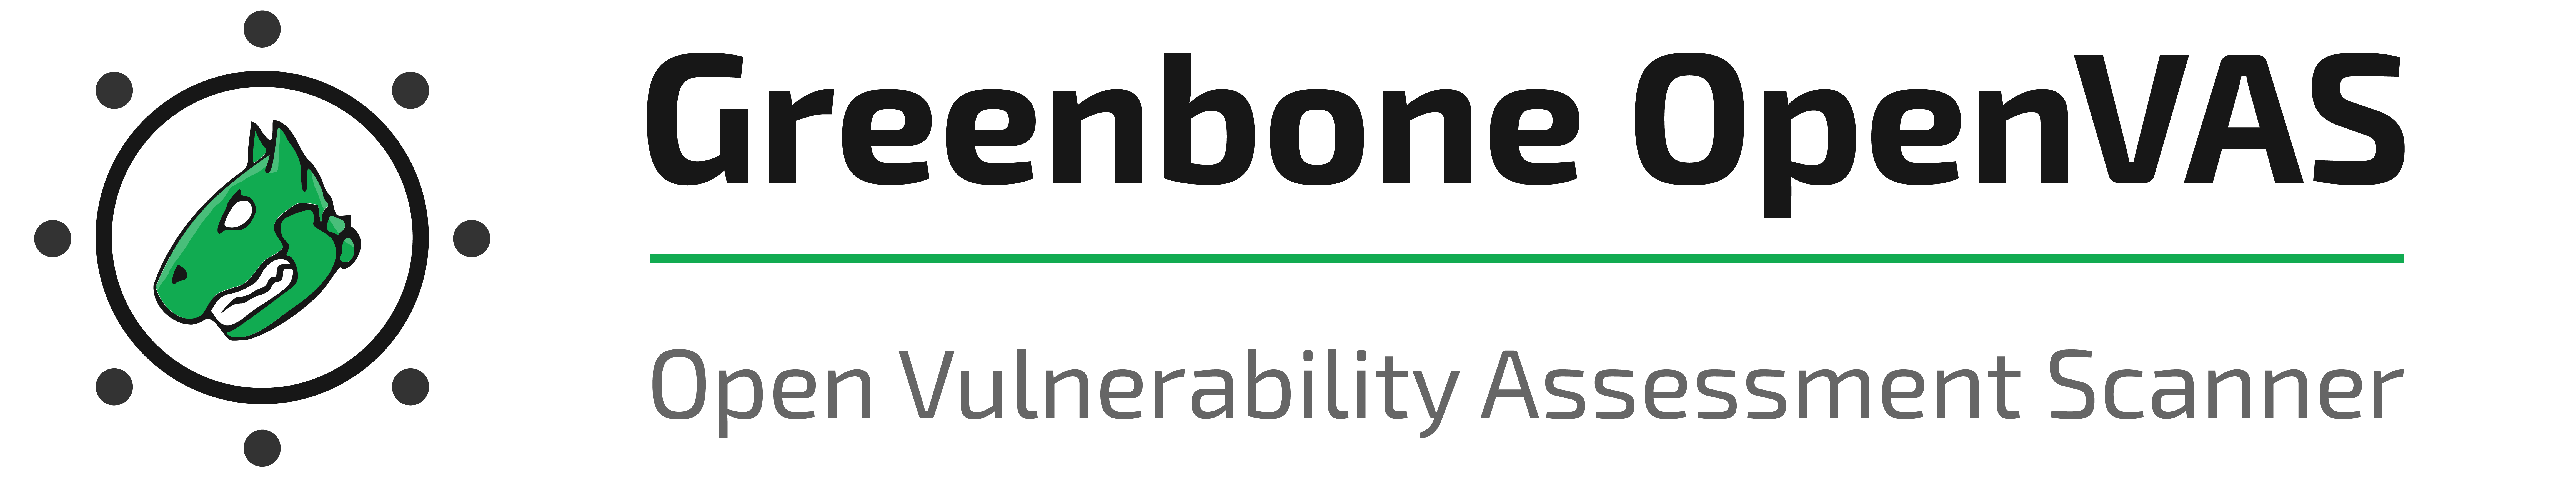
\includegraphics[width=0.8\textwidth]{img/greenbone_logo.png}
    \caption{Nuovo logo del progetto Greenbone OpenVAS}
\end{figure}

\section{Modello di business}
Greenbone OpenVAS e GVM ricevono aggiornamenti di sicurezza e configurazioni attraverso due \emph{feed}, entrambi mantenuti da Greenbone:
\label{feed}

\begin{itemize}
    \item \textbf{Greenbone Community Feed}: canale di aggiornamenti gratuito e \emph{open source}, contenente configurazioni di scansione minimali, liste di porte e reportistica essenziale. Questo \emph{feed} include esclusivamente i test di vulnerabilità più critici e importanti. Gli aggiornamenti sono distribuiti giornalmente secondo una politica \emph{best effort}, senza garanzie specifiche.
    \item \textbf{Greenbone Enterprise Feed}: canale di aggiornamenti a pagamento, pensato per i clienti \emph{enterprise}. Include tutti i test di vulnerabilità disponibili, configurazioni di scansione avanzate e reportistica dettagliata. Il servizio è garantito da SLA\footnote{\emph{Service Level Agreement}: contratto che assicura standard minimi di qualità e disponibilità.}.
\end{itemize}

Il progetto è finanziato principalmente tramite la sottoscrizione al \emph{feed} \emph{enterprise}. Inoltre, Greenbone offre anche \emph{hardware appliance}\footnote{Dispositivi fisici progettati per eseguire una specifica funzione, ottimizzati per tale scopo.}, \emph{virtual appliance}\footnote{Sistemi virtuali progettati per essere eseguiti in ambienti di virtualizzazione.} e una soluzione SaaS gestita direttamente dall'azienda.

\subsection{Greenbone Operating System (GOS)}
Il Greenbone Operating System è il sistema operativo che alimenta le \emph{appliance} fornite da Greenbone. Si tratta di un insieme di strumenti grafici e TUI\footnote{\emph{Terminal User Interface}} che semplificano la gestione e la manutenzione del sistema. GOS integra anche supporto commerciale da parte di Greenbone e vari miglioramenti all'esperienza utente.

\section{Architettura}
L'architettura del framework Greenbone Vulnerability Management (GVM) si compone di numerosi componenti interconnessi, ognuno con un ruolo specifico nel sistema.

\subsection{gvmd}
Il demone UNIX \texttt{gvmd} costituisce il cuore del framework GVM. Si occupa della gestione e dell'interconnessione tra tutte le principali componenti di basso livello, fornendo un'API di gestione operabile tramite il protocollo \textbf{Greenbone Management Protocol (GMP)}.
\label{gmp}

Le principali funzioni del \texttt{gvmd} includono:
\begin{itemize}
    \item Comunicazione con lo scanner OpenVAS tramite il protocollo \textbf{Open Scanner Protocol (OSP)}.
    \item Gestione del database (generalmente un'istanza di PostgreSQL) per la memorizzazione di dati ricevuti dai feed configurati, risultati delle scansioni, utenti e ruoli interni al framework GVM.
    \item Funzione di server web per \textbf{GSA}, l'interfaccia web ufficiale di Greenbone, attraverso la quale si gestisce il sistema.
\end{itemize}

Il demone \texttt{gvmd} consente inoltre un'operatività diretta tramite l'API offerta sotto protocollo GMP, permettendo la creazione di strumenti personalizzati di automazione o interfacce alternative.

\begin{figure}[h!]
    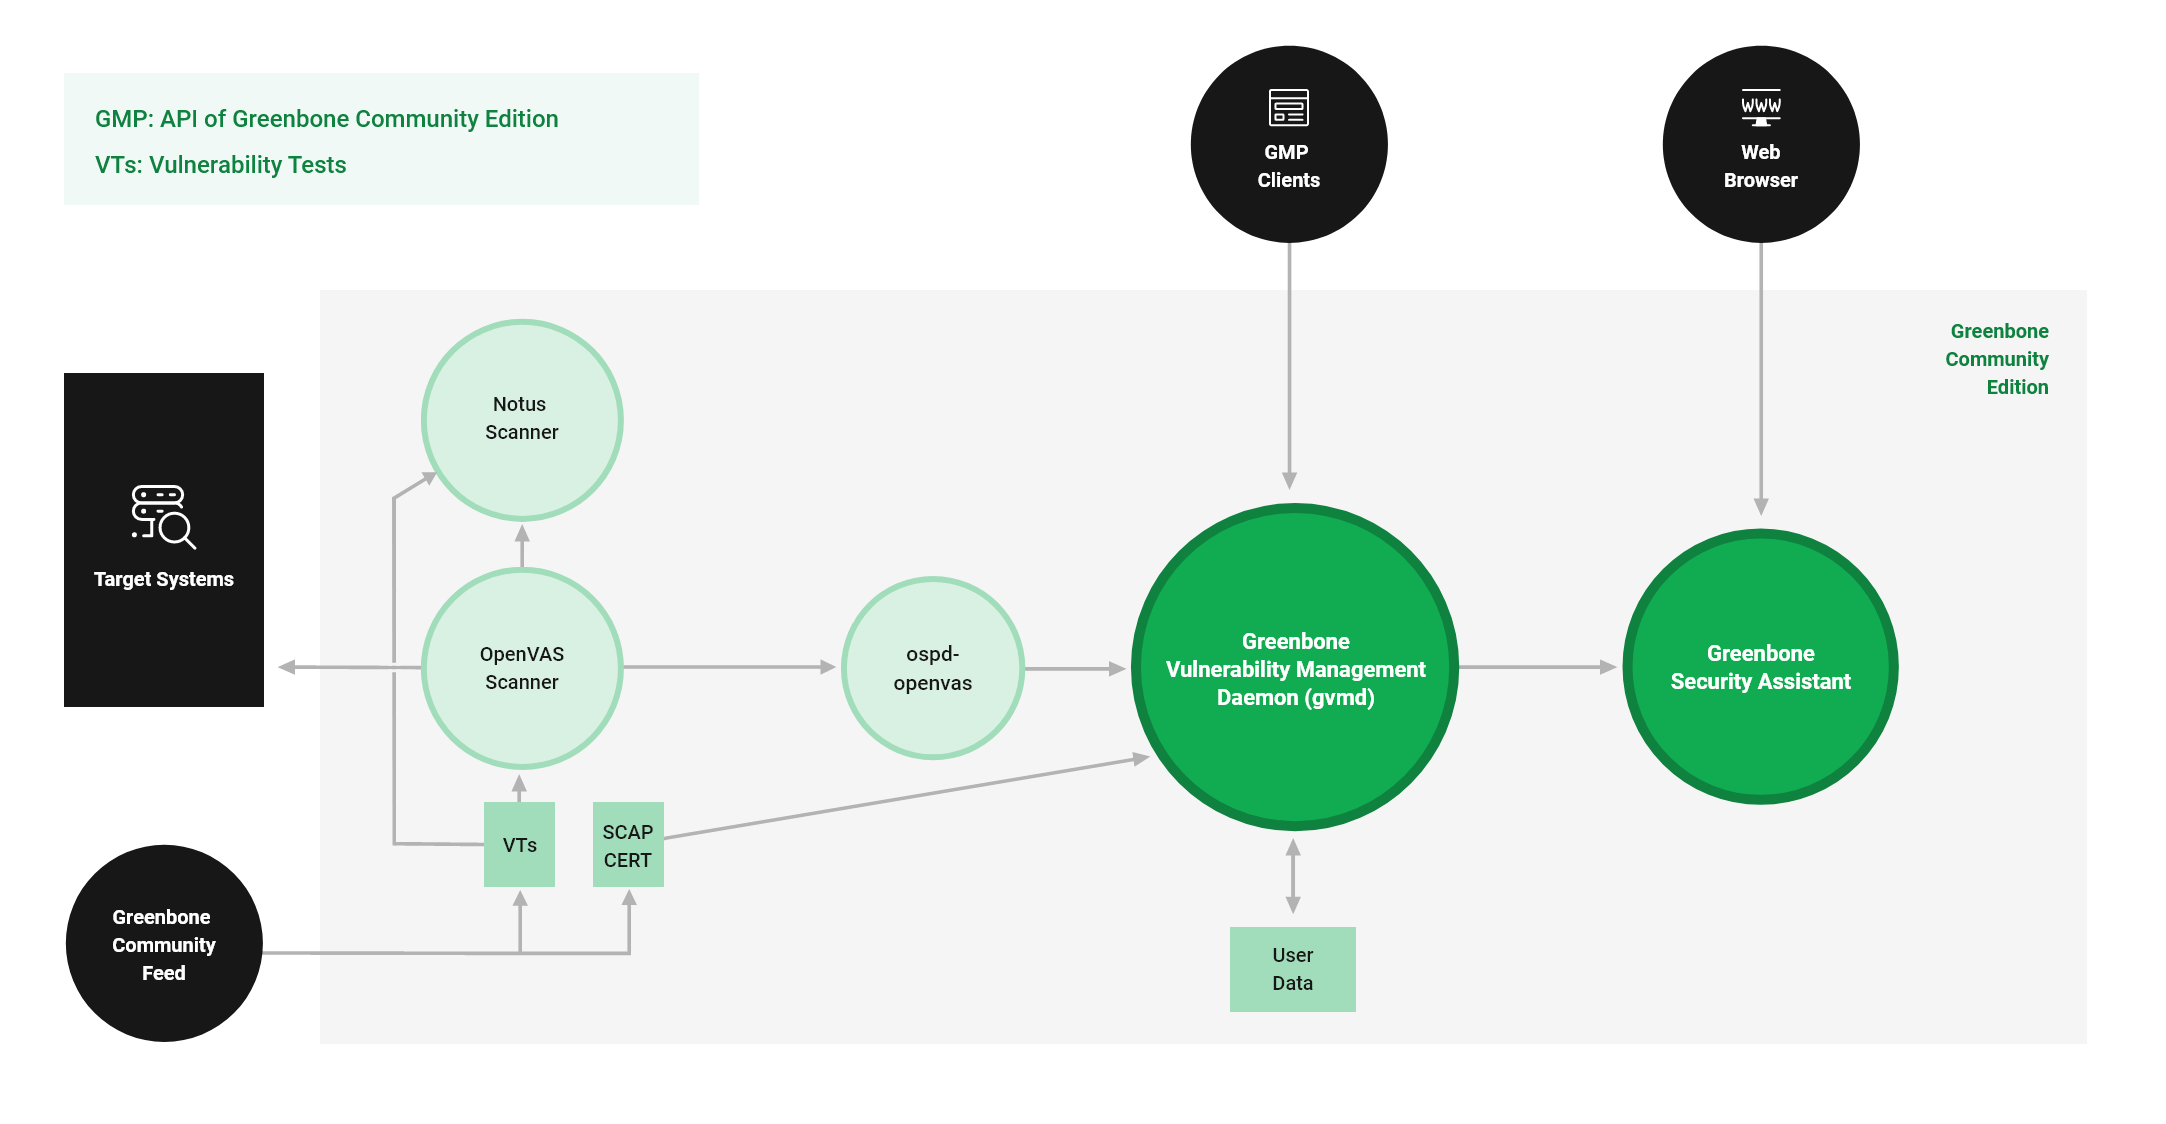
\includegraphics[width=\textwidth]{img/greenbone-community-22.4-architecture.png}
    \caption{Architettura della release 22.4 di Greenbone}
\end{figure}

\subsection{Greenbone Security Assistant (GSA)}
\textbf{Greenbone Security Assistant (GSA)} è l'interfaccia web nativa di Greenbone, sviluppata con React, progettata per l'interazione diretta dell'utente tramite browser.

Il web server \texttt{gsad} eroga \textbf{GSA} e svolge anche funzioni di backend. \`E interamente realizzato in linguaggio C standard.

\subsection{Vulnerability Test (VT)}
Gli scanner eseguono applicazioni sui sistemi bersaglio per identificare vulnerabilità. Questi programmi, detti \textbf{Vulnerability Test (VT)}, o talvolta \textbf{Network Vulnerability Test (NVT)}, sono scritti nel linguaggio \textbf{NASL}.

\textbf{NASL (NASL Attack Scripting Language)} \`e un linguaggio di dominio specifico (DSL), interpretato, progettato per definire test mirati alla rilevazione di vulnerabilità su dispositivi di rete. NASL offre funzioni integrate per semplificare la scrittura di questi script.

Gli script NASL vengono eseguiti principalmente durante le scansioni di OpenVAS, ma possono anche essere eseguiti direttamente tramite l'interprete NASL incluso nel framework (\texttt{openvas-nasl}).

\subsection{SCAP (CVE, CPE)}
\textbf{SCAP (Security Content Automation Protocol)} è uno standard aperto sviluppato nei primi anni 2000 dal \textbf{NIST}\footnote{National Institute of Standards and Technology} statunitense, un riferimento importante nel campo della cybersecurity. Lo standard SCAP regola e automatizza i processi di valutazione della sicurezza delle risorse informatiche.

SCAP comprende un insieme di standard, definiti \textbf{componenti}, tra cui:
\begin{itemize}
    \item \textbf{Common Vulnerabilities and Exposures (CVE)}: fornisce identificativi univoci per le vulnerabilità note.
    \item \textbf{Common Platform Enumeration (CPE)}: standardizza la descrizione dell'inventario informatico (applicazioni, servizi software, sistemi operativi, hardware).
    \item \textbf{Common Configuration Enumeration (CCE)}: identifica univocamente diverse configurazioni di sistema.
    \item \textbf{Common Vulnerability Scoring System (CVSS)}: valuta la severità di una vulnerabilità con un punteggio compreso tra 0 e 10.
\end{itemize}

GVM utilizza i feed menzionati nella sezione \ref{feed} per aggiornare continuamente i dati SCAP necessari, in particolare quelli relativi a \textbf{CVE} e \textbf{CPE}. Il framework include anche un calcolatore del punteggio \textbf{CVSS} accessibile tramite \textbf{GSA}.

\subsection{OpenVAS e Notus}
\label{notus}
Lo scanner principale del sistema è \textbf{OpenVAS}, ma è disponibile anche un altro componente chiamato \textbf{Notus}. Quest'ultimo è un modulo Python che ottimizza e razionalizza l'esecuzione degli script NASL.

\label{openvasd}
A partire dalla versione 23.0 di OpenVAS, è stato introdotto \texttt{openvasd}, un nuovo demone che integra le funzionalità di OpenVAS (scanner), Notus (ottimizzazione degli script NASL) e \texttt{ospd-openvas} (intermediario che utilizza il protocollo \textbf{OSP} per la comunicazione tra scanner e \texttt{gvmd}).

Il demone \texttt{openvasd} è stato riscritto in Rust per migliorarne le prestazioni e la manutenibilità. Inoltre, l'API OSP sarà sostituita da una API HTTP.

\section{Funzionalità peculiari}
Seguono ora alcune funzionalità e terminologie caratteristiche del sistema OpenVAS.

\subsection{Scanner CVE / Prognosi}
\label{cve}
In aggiunta allo scanner vero e proprio di OpenVAS, Greenbone mette a disposizione un ulteriore scanner ``fittizio'', detto \textbf{CVE}.

Questo scanner effettua una prognosi della sicurezza del sistema basandosi sulle informazioni già raccolte in una precedente scansione effettuata da OpenVAS. Pertanto, può diventare operativo solo successivamente a una scansione completa ed efficace.

In particolare, se OpenVAS ha popolato i dati CPE del sistema in esame, lo scanner CVE utilizza tali informazioni per stimare la sicurezza attuale confrontando i CPE identificati con quelli dei CVE disponibili.

Si noti che questa è una scansione ``fittizia'', poiché non interagisce direttamente con il sistema in oggetto, il quale potrebbe essere stato aggiornato nel frattempo o addirittura dismesso. Di conseguenza, i risultati dello scanner possono includere un maggior numero di falsi positivi rispetto a una scansione reale eseguita da OpenVAS. Tuttavia, questa ``scansione'' è quasi istantanea, a differenza di OpenVAS che richiede un tempo significativo, oltre a risorse computazionali e di rete, specialmente in ambienti con un grande numero di host da analizzare.

\subsection{Quality of Detection (QoD)}
\label{qod}
La \textbf{Quality of Detection (QoD)} è un valore compreso tra 0 e 100 che rappresenta l'affidabilità del processo di rilevamento delle vulnerabilità per uno specifico test (VT). Questo parametro funge da metrica euristica per stimare la precisione nel determinare se un sistema è effettivamente vulnerabile.

Ecco alcuni esempi dei valori di QoD dati a diversi scenari:
\begin{itemize}
    \item I risultati verificati tramite \emph{exploit} eseguiti con successo ricevono un QoD del 100\%.
    \item Controlli remoti attivi che evidenziano chiaramente la presenza della vulnerabilità ricevono un punteggio tra il 95 e il 99\%.
    \item Controlli basati sulla versione degli applicativi, con risposte dettagliate fino al livello di patch, ricevono un QoD dell'80\%.
    \item Controlli che dipendono da circostanze ambientali più o meno aleatorie ottengono un valore del 70\%.
    \item Situazioni in cui un firewall potrebbe impersonare il sistema bersaglio ottengono un QoD del 50\%.
    \item Applicazioni che non forniscono dettagli precisi sulla versione generano un QoD del 30\%.
    \item Valori inferiori di QoD indicano vulnerabilità potenziali senza conferma diretta della loro presenza.
\end{itemize}

Il valore predefinito utilizzato da GSA è 70, ritenuto da Greenbone una buona soglia euristica di compromesso, sotto la quale si trovano spesso falsi positivi.

\subsection{Override}
\label{override}
Le regole interne di Greenbone riguardanti la severità e la qualità dei risultati possono essere modificate dall'utente tramite un cosiddetto \emph{override}. Questa funzionalità permette di ridefinire le priorità dello scanner per adattarle alle specifiche policy dell'ambiente in esame.

\subsection{Powerfilter}
\label{powerfilter}
OpenVAS è spesso utilizzato per gestire grandi quantitativi di dati, come task di scansione, risultati, vulnerabilità, host trovati e obiettivi.

Per facilitare la gestione avanzata dei dati, OpenVAS include un linguaggio di query specifico chiamato \textbf{Powerfilter}, integrato persino a livello di protocollo GMP. Powerfilter consente di filtrare e manipolare i risultati in modo dettagliato attraverso diverse regole. Tra le funzionalità principali:
\begin{itemize}
    \item Selezione del valore minimo di QoD (vedi \ref{qod}).
    \item Applicazione o esclusione degli override definiti dall'utente (vedi \ref{override}).
    \item Filtraggio basato su punteggi di severità, soluzioni, host, porta, protocollo e altre informazioni ritornate.
    \item Controllo della paginazione (numero di risultati per pagina, pagina specifica, ecc.).
    \item Ordinamento dei risultati in base a diversi criteri (valore, ordine ascendente o discendente, ecc.).
\end{itemize}

\section{Installazione}
Laddove l'edizione Enterprise viene solitamente fornita preinstallata e preconfigurata nelle \emph{appliance}, eliminando di fatto la necessità di un'installazione manuale, l'edizione gratuita deve essere invece installata e configurata dall'utente in base alle proprie esigenze.

Sono disponibili due principali modalità di installazione e gestione del sistema:

\begin{itemize}
    \item \textbf{Compilazione da sorgenti}: l'utente deve scaricare il codice sorgente dalle \emph{repository} pubbliche e procedere manualmente alla compilazione. Questo approccio non è consigliato per ambienti di produzione, a causa del rischio di instabilità nell'ultima versione disponibile.
    
    \item \textbf{Greenbone Community Containers}: i singoli componenti del framework Greenbone (già descritti in \ref{greenbone-architecture}) sono segregati in immagini Docker separate, garantendo riproducibilità di versioni rilasciate e funzionalità. Grazie poi a \texttt{docker-compose}, i container possono essere orchestrati e gestiti ricostruendo l'architettura generale.
    \label{greenbone-community-containers}

    Maggiori dettagli su questa tecnica di deployment (\ref{compose-architecture}) e sull'uso di Docker (\ref{docker}) e Docker Compose (\ref{docker-compose}) sono forniti nelle sezioni del capitolo relativo all'installazione del progetto finale.
\end{itemize}

Alcune distribuzioni Linux offrono pacchetti precompilati nelle loro \emph{repository} native. Tuttavia, Greenbone non garantisce alcun tipo di supporto ufficiale per eventuali errori derivanti dall'uso di queste edizioni, poiché non è coinvolta nel processo di compilazione.

\section{Interoperabilità e protocollo GMP}
\label{libraries}
Come descritto nella sezione \ref{gmp}, il demone di sistema di OpenVAS può interfacciarsi non solo con i client nativi (come GSA), ma anche con client originali e personalizzati mediante il protocollo \textbf{GMP}.

GMP, un dialetto XML personalizzato, funziona attraverso un processo di richiesta-risposta standardizzato con messaggi e attributi specifici. La comunicazione avviene tramite una \textbf{socket UNIX}, accessibile in diversi modi:

\begin{itemize}
    \item \textbf{Interfacciamento manuale}: gli sviluppatori possono utilizzare strumenti dedicati per creare manualmente i messaggi XML conformi agli standard Greenbone.

    \item \texttt{python-gvm}: una libreria Python ufficiale sviluppata da Greenbone che semplifica la comunicazione con la socket. Questa libreria offre diversi vantaggi:
    \begin{itemize}
        \item Automatizzazione della creazione dei messaggi XML, richiedendo solo i parametri necessari.
        \item Gestione integrata dell'autenticazione, necessaria di fatto per tutti i messaggi GMP.
        \item Supporto per la gestione degli errori attraverso il meccanismo delle eccezioni di Python.
        \item Idratazione automatica delle risposte in oggetti Python utilizzando \texttt{lxml}, facilitando la manipolazione dei documenti XML restituiti.
    \end{itemize}

    \item \texttt{gvm-tools}: uno strumento pensato per gli amministratori di sistema che desiderano gestire OpenVAS da linea di comando, automatizzando operazioni comuni. Questo strumento si basa su \texttt{python-gvm}, agendo come un \emph{wrapper} per la libreria.
\end{itemize}

\section{Motivazioni alla base della scelta}
I principali fattori che motivano la scelta di OpenVAS come backend di scansione del progetto includono:

\begin{itemize}
    \item \textbf{Disponibilità di una versione gratuita}: OpenVAS offre una soluzione senza costi di licenza, permettendo all'azienda di occuparsi solo della predisposizione e manutenzione dell'hardware necessario. Tuttavia, è importante notare che la versione gratuita non include tutti i test di sicurezza disponibili, rendendo necessaria una valutazione aggiuntiva per determinare se i dati forniti siano in linea con il \emph{threat model} dell'azienda.
    
    \item \textbf{Open source}: OpenVAS è un progetto open source, consentendo la visione e la verifica del codice sorgente. Questo riduce il rischio di utilizzare componenti non documentati o poco trasparenti.

    \item \textbf{Librerie ufficiali}: Greenbone offre strumenti ufficiali che semplificano l'interazione con il sistema OpenVAS e implementano un ampio spettro di funzionalità del protocollo GMP.
\end{itemize}